\section{Konzeption}\label{konzeption}

In diesem Kapitel werden einige Konzeptionsentwürfe dargestellt und erläutert. 
Zuerst wird der allgemeine Architekturentwurf präsentiert. Im Anschluss folgen die Entwürfe für Server, Datenbank, Client und Schnittstellen.

\subsection{Allgemeiner Architekturentwurf}\label{allgemeiner_Architekturentwurf}

In diesem Unterkapitel wird der allgemeine Architekturentwurf erläutert.
\\
\\
Für das Projekt wird eine Client-Server-Architektur gewählt, da aus der Anforderungsanalyse hervorgeht, dass die Anwendung auf möglichst vielen Geräten standortunabhängig lauffähig sein soll. Außerdem soll in Zukunft die Möglichkeit bestehen, dass eine App eingebunden werden kann.
\\
\\

\begin{figure}[htb]
	\centering
	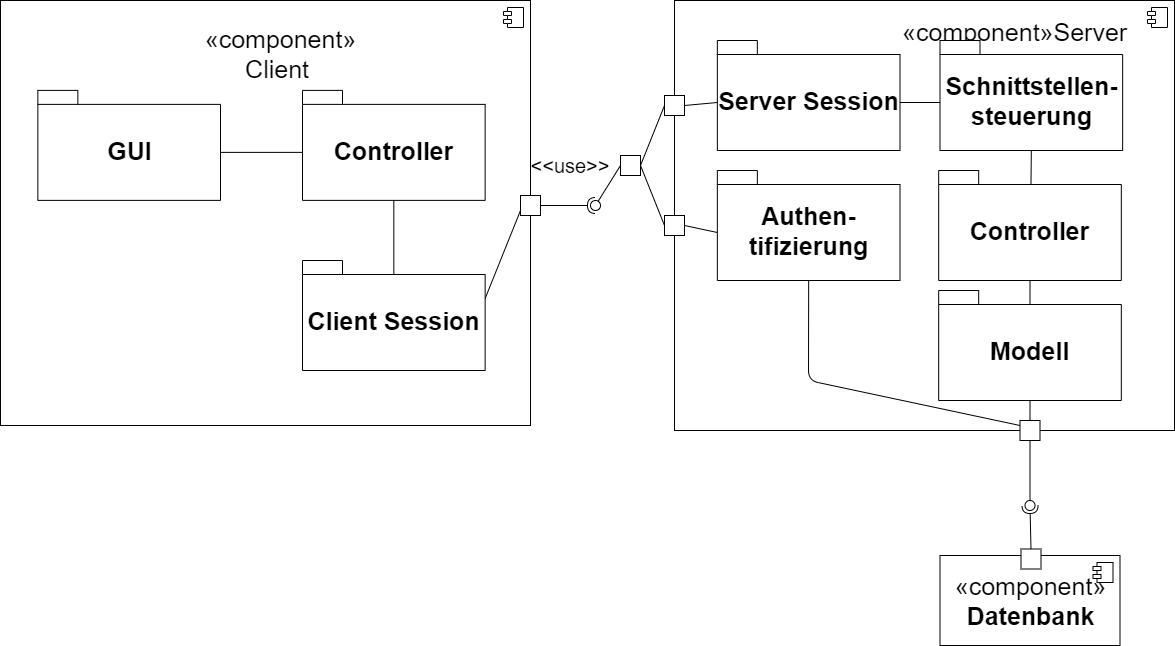
\includegraphics[width=1\textwidth,angle=0]{abb/Komponentendiagramm}
	\caption[Komponentendiagramm]{Komponentendiagramm}
	\label{fig:Komponentendiagramm}
\end{figure}

Die Abbildung~\ref{fig:Komponentendiagramm} zeigt ein Komponentendiagramm, mit folgenden drei Komponenten Client, Server und Datenbank. 
Die Darstellung ist eine vereinfachte Abbildung, diese dient dazu einen ersten Überblick über das zu entwerfende System zu erhalten. 
\\
\\
Der Client enthält drei Pakete GUI, Controller und Client Session. 
\\
GUI (Graphical User Interface) beinhaltet die Grafische Benutzeroberfläche.
\\
Sobald ein Benutzer eine Eingabe tätigt, wird diese an den Controller gesendet. Der Controller ist dafür zuständig, die Eingaben zu prüfen, weiterzuleiten, zu ändern usw.. Sollte der Controller Daten vom Server benötigen, wird eine Session (Verbindung) zum Server aufgebaut, dafür ist das Paket Client Session zuständig.
\\
\\
Der Server beinhaltet fünf Pakete Server Session, Authentifizierung, Schnittstellensteuerung, Controller und Modell. 
\\
Sollte der Benutzer bislang noch kein Account angelegt haben oder die Zugriffsberechtigung (Token) ist abgelaufen, muss eine neue Authentifizierung durchgeführt werden. Hierfür ist das Paket Authentifizierung zuständig.
\\
Ansonsten wird mithilfe einer Server Session eine Verbindung aufgebaut. 
 \\
Das Paket Schnittstellensteuerung verwaltet eingehende Anfragen und leitet diese an den Controller weiter. Das Paket Controller steuert die eingehenden Anfragen. Sobald Anfragen Daten ändern, löschen, hinzufügen oder abfragen, sendet der Controller diese an das Paket Modell. Die Pakete Authentifizierung und Modell können eine Verbindung zur Datenbank aufbauen.

\subsection{Entwurf der Datenbank}\label{entwurf_der_Datenbank}

In diesem Kapitel werden die einzelnen Entwurfsschritte, die zum Erstellen der Datenbank notwendig sind, erläutert. 
Wie bereits in Kapitel~\ref{sQL-Datenbank} erwähnt, wird eine rationale Datenbank umgesetzt.

\subsubsection{Normalisierung der Datenbank}\label{normalisierung}

Es liegt nach der Anforderungsanalyse folgende Ausgangssituation vor. Nachfolgende Daten sollen unter anderem gespeichert werden:
Benutzername, Passwort, Benutzerrolle, Selbstbedienungsstandname, Datum, Warenname, Preis(€), Wareneingang, gezählte Waren, verkaufte Waren, Einnahmen(€).
\\
\\
Aus diesen Daten wird ein Entity-Relationship-Modell (ER-Modell) erstellt, dieses beinhaltet Entitäten, Attribute, Beziehungen, Primärschlüsseln, zusammengesetzte Primärschlüssel und Fremdschlüssel.
Aus dem ER-Modell werden im Anschluss Tabellen erstellt.
\\
Eine Entität (Rechteck) beschreibt ein Objekt, daraus wird später der Tabellenname. Die Attribute (Ellipsen) werden in Tabellenspalten überführt.
\\
Ein Primärschlüssel (unterstreichendes Attribut) dient dazu, die einzelnen Datensätze auch Tupel genannt eindeutig zu identifizieren.
Bei einem zusammengesetzten Primärschlüssel werden zwei oder mehr Attribute zur eindeutigen Erkennung eines Tupels verwendet.
Der Fremdschlüssel verweist auf ein anderes Attribute, dieses muss ein Primärschlüssel sein. Dadurch können Tabellen miteinander in Beziehung (Raute) gebracht werden.

\begin{figure}[htb]
	\centering
	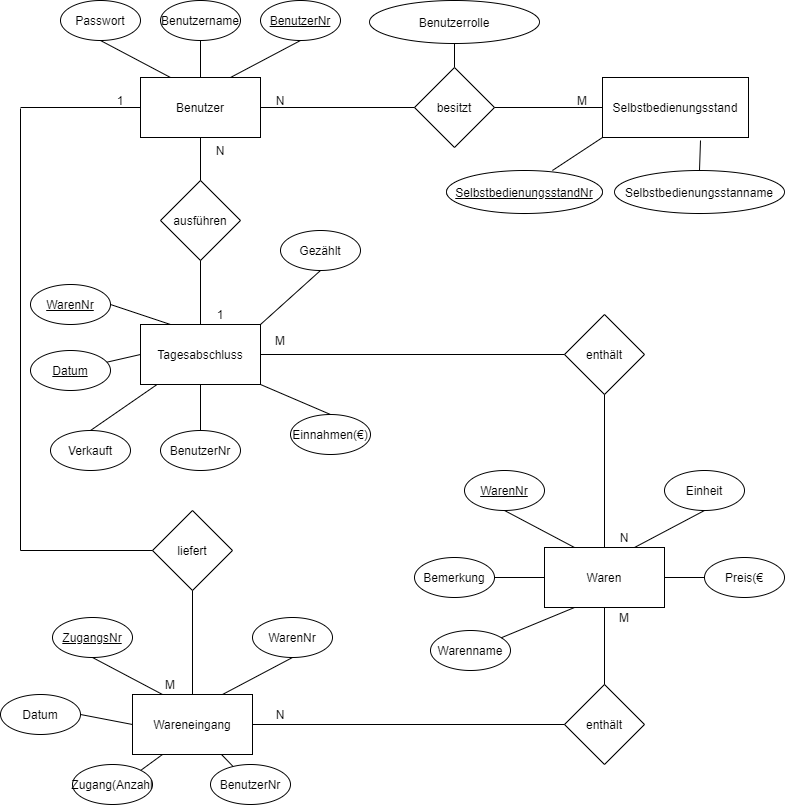
\includegraphics[width=1\textwidth,angle=0]{abb/ER-Modell}
	\caption[ER-Modell]{ER-Modell}
	\label{fig:ER Modell}
\end{figure}


In der Abbildung~\ref{fig:ER Modell} ist das erstellte ER-Modell abgebildet. Daraus werden die Tabellen abgeleitet. 

\cite{DBREdun} empfiehlt es, eine Datenbank so zu gestalten das \glqq Redundanzen, Inkonsistenzen und Anomalien\grqq{} vermieden werden. 
Dieses soll mithilfe der Normalformen umgesetzt werden.
Es existieren bis zu fünf Normalformen, in der Praxis werden oftmals nur die ersten drei Normalformen gebildet, erwähnt \cite{DB2}.
Es sollen nachfolgend drei aufeinander aufbauende Normalisierungschritte durchgeführt werden.

\cite{relaDatenbank} zufolge sollten die folgenden Datenbankanforderungen eingehalten werden:

\begin{itemize}
	\itemsep0pt
	\item Eindeutige Struktur, jeder Datensatz muss eindeutig zu identifizieren sein.
	\item Redundanzfrei, nach Möglichkeit sollten keine Daten mehrfach vorhanden sein.
	\item Keine Inkonsistenzen, keine Widersprüchlichkeit zwischen den Daten.
\end{itemize} 


Die Voraussetzung für die erste Normalform ist, dass alle Tabellenspalten gleichartige Werte enthalten und alle Daten atomar sind.
Das heißt, eine Tabellenspalte darf keine unterschiedlichen Typen enthalten, z.B. Betrag in Euro und Betrag in Cent. 
Außerdem müssen die Daten atomar sein, es ist nicht erlaubt mehrere Werte in einem Feld zu haben z.B. Straße, Postleitzahl, Ort.
\\
\\
Der Autor \cite{DB2} schreibt, sobald eine Tabelle in der ersten Normalform und jedes Nichtschlüsselattribut vom Primärschlüssel funktional abhängig ist, befindet sich die Tabelle in der zweiten Normalform. Dieses trifft bereits zu, z. B. der Benutzername ist abhängig von der BenutzerNr..
\\
\\
Bei der Erstellung der Tabellen wird darauf geachtet das diese direkt in der 2. Normalform vorliegen. 

\begin{table}[H]
	\centering
	\begin{tabular}{|c|c|c|}
		\hline
		\underline{BenutzerNr} & Benutzername & Passwort \\
		\hline
		1 & Christine &  12345\\
		\hline
		2 & ADE &  asdfg\\
		\hline
		3 & Hugo &  yxcvb\\
		\hline
	\end{tabular}
	\caption{Die Tabelle Benutzerdaten in der 2. Normalform.}
	\label{tab: Benutzerdaten 2.NF}
\end{table}

\begin{table}[H]
	\centering
	\begin{tabular}{|c|c|}
		\hline
		\underline{SelbstbedienungsstandNr} & Selbstbedienungsstandname \\
		\hline
		1 & Eierhütte \\
		\hline
		2 & Kartoffelhaus \\
		\hline
		3 & Stand1 \\
		\hline
	\end{tabular}
	\caption{Die Tabelle Selbstbedienungsstand in der 2. Normalform.}
	\label{tab: Selbstbedienung 2.NF}
\end{table}

\begin{table}[H]
	\centering
	\begin{tabular}{|c|c|c|}
		\hline
		\underline{SelbstbedienungsstandNr} & \underline{BenutzerNr} & Benutzerrolle \\
		\hline
		1 & 1 &  Admin\\
		\hline
		2 & 1 &  User\\
		\hline
		3 & 2 &  Admin\\
		\hline
		3 & 3 &  Admin\\
		\hline
	\end{tabular}
	\caption{Die Tabelle Selbstbedienungsstand-Nutzer in der 2. Normalform.}
	\label{tab: Selbstbedienung-Nutzer 2.NF}
\end{table}

Die Tabellen ~\ref{tab: Benutzerdaten 2.NF}, ~\ref{tab: Selbstbedienung 2.NF} und ~\ref{tab: Selbstbedienung-Nutzer 2.NF} beinhalten die Benutzerdaten und Selbstbedienungsstanddaten. Es wird davon ausgegangen das ein Selbstbedienungsstand mehrere Benutzer haben kann, gleichzeitig kann ein Nutzer mehrere Selbstbedienungsstände betreiben, dieses wird mithilfe der Tabelle~\ref{tab: Selbstbedienung-Nutzer 2.NF} umgesetzt.

\begin{table}[H]
	\centering
	\begin{tabular}{|c|c|c|c|c|}
		\hline
		\underline{WarenNr} & Warenname & Einheit & Preis(€)& Bemerkung \\
		\hline
		1 & Ei & Stück &  0,20 & \\
		\hline
		2 & Kartoffeln & KG & 5 & Sorte Annabelle \\
		\hline
	\end{tabular}
	\caption{Die Tabelle Waren in der 2. Normalform.}
	\label{tab: Waren 2.NF}
\end{table}


\begin{table}[H]
	\centering
	\begin{tabular}{|c|c|c|c|c|}
		\hline
		\underline{WareneingangsNr} & Datum & Wareneingang(Anzahl) & WarenNr & BenutzerNr \\
		\hline
		1 & 25.07.2021 & +100 & 2 & 1 \\
		\hline
		2 & 25.07.2021  & +80 & 1 & 1 \\
		\hline
		3 & 26.07.2021  & +60 & 2 & 1 \\
		\hline
		4 & 26.07.2021  &+5 & 2 &  2\\
		\hline
	\end{tabular}
	\caption{Die Tabelle Wareneingang in der 2. Normalform.}
	\label{tab: Wareneingang 2.NF}
\end{table}


\begin{table}[H]
	\centering
	\begin{tabular}{|c|c|c|c|c|c|}
		\hline
		\underline{Datum} & \underline{WarenNr} & BenutzerNr & Gezählt & Verkauft & Einnahmen(€) \\
		\hline
		25.07.2021 & 1 & 1 & 231 & 251 & 50,20 \\
		\hline
		26.07.2021 & 1 & 1 & 52 & 239 & 47,80 \\
		\hline
		26.07.2021 & 2 & 1 & 3 & 2 & 10 \\
		\hline
	\end{tabular}
	\caption{Die Tabelle Tagesabschluss in der 2. Normalform.}
	\label{tab: Tagesabschluss 2.NF}
\end{table}

In dieser Tabelle~\ref{tab: Tagesabschluss 2.NF} ist die Spalte BenutzerNr nachträglich hinzugefügt worden, dadurch lässt sich eindeutig erkennen wer den Tagesabschluss ausgeführt hat.
\\


Die Tabelle~\ref{tab: Selbstbedienung-Nutzer 2.NF} und Tabelle~\ref{tab: Waren 2.NF} befinden sich noch nicht in der dritten Normalform, die restlichen Tabellen befinden sich in der dritten Normalform, aus diesem Grund werden die Tabellen nachfolgend nicht mehr aufgeführt.
\\
\\
Eine Tabelle ist in der dritten Normalform, sobald diese sich in der zweiten Normalform befindet und \grqq kein Nichtschlüsselattribut transitiv von einem Kandidatenschlüssel abhängt\grqq{} \cite{DB3}. Das heißt, indirekte Abhängigkeiten sollen vermieden werden.


\begin{table}[H]
	\centering
	\begin{tabular}{|c|c|c|}
		\hline
		\underline{SelbstbedienungsstandNr} & \underline{BenutzerNr} & Benutzerrolle \\
		\hline
		1 & 1 &  1\\
		\hline
		2 & 1 &  2\\
		\hline
		3 & 2 &  1\\
		\hline
		3 & 3 &  1\\
		\hline
	\end{tabular}
	\caption{Die Tabelle Selbstbedienungsstand-Nutzer in der 3. Normalform.}
	\label{tab: Selbstbedienung-Nutzer 3.NF}
\end{table}


\begin{table}[H]
	\centering
	\begin{tabular}{|c|c|}
		\hline
		\underline{\underline{RollenNr}} & Benutzerrollename \\
		\hline
		1 & Admin  \\
		\hline
		2 & User \\
		\hline
	\end{tabular}
	\caption{Die Tabelle Benutzerrollen-Nutzer in der 3. Normalform.}
	\label{tab: Benutzerrolle 3.NF}
\end{table}

Die Tabelle~\ref{tab: Benutzerrolle 3.NF} beinhaltet die aktuellen Benutzerrollen, aktuell die Rolle Admin und User, allerdings lassen sich leicht neue Rollen hinzufügen und bestehende Rollen verändern. 
\\
\\
Im Anhang~\ref{3NF} sind alle Tabellen nochmals in der dritten Normalform aufgeführt.


\subsection{Entwurf des Servers}\label{entwurf_des_Serversr}

Anhand eines Paketdiagramms wird der Entwurf des Servers erläutert.
\cite{Server1} beschreibt ein Paket, als eine Sammlung an inhaltlich zusammengehörigen Klassen. Klassen sind Vorlagen, \glqq Sie sind Vorlagen, aus denen Objekte erzeugt werden. Objekte haben Eigenschaften und Methoden.\grqq{} schreibt \cite{Server2}.
\\
\\
Aus den zuvor erstellten Tabellen lassen sich bereits einige Pakete ableiten. Beispielweise das Paket, Repository, in diesem Paket werden alle Klasse gebündelt die für Datenbankenabfragen zuständig sind. 

\begin{figure}[htb]
	\centering
	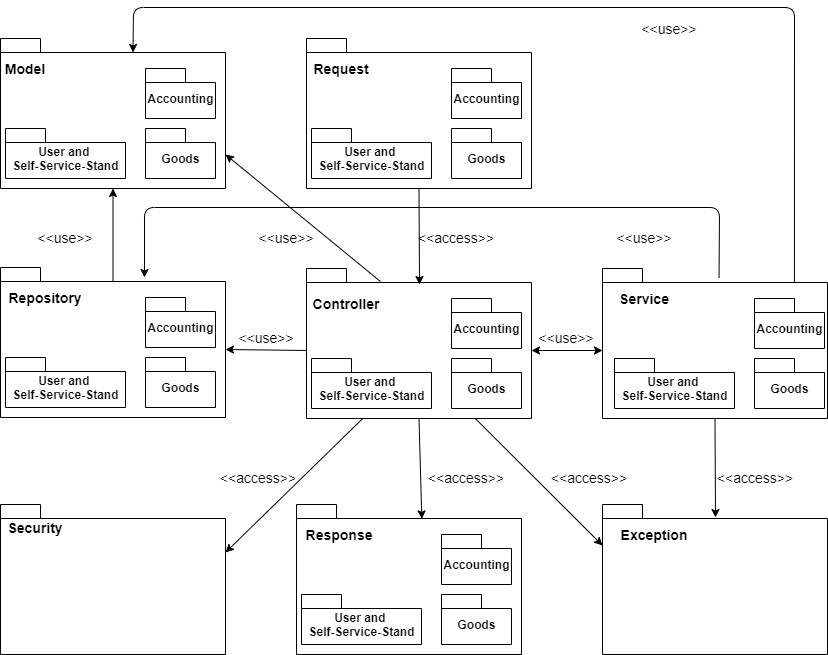
\includegraphics[width=1\textwidth,angle=0]{abb/Paketdiagramm}
	\caption[Paketdiagramm des Servers]{Paketdiagramm des Servers}
	\label{fig:AB_Paketdiagramm_Server}
\end{figure}


In der Abbildung ~\ref{fig:AB_Paketdiagramm_Server} ist das erstellte Paketdiagramm abgebildet, anhand des Paketdiagramms wird der Aufbau des Servers erläutert. 
\\
\\
Das Paket Request (Anfrage) enthält Klassen, die die Struktur der Anfragen an eine Schnittstelle festlegen. Beispielhaft enthält die Klasse Goods im Unterpaket goods unter anderem folgende Variablen goodsName, goodsPrice usw.. Sobald eine Anfrage an eine Schnittstelle gesendet wird, muss die vorgebende Struktur eingehalten werden. Das heißt zum Beispiel, gleiche Namen und vorgebende Datentypen (int, String usw.).
\\
Eines der wichtigsten Pakete ist das Controller Paket. Alle eingehenden Anfragen an die REST-API werden von einer Klasse im Paket Controller entgegengenommen. Der Controller entscheidet, was mit einer eingehenden Anfrage geschehen soll, zuerst prüft der Controller die eingehenden Daten auf Korrektheit. Anschließend steuert der Controller den Datenfluss und leitet die Daten weiter an die zuständigen Serviceklassen, Securityklassen oder Exeptionklassen.
\\
\\
Im Paket Response(Antwort) sind Klassen enthalten, die die Struktur der Ausgabennachrichten, die an einen Anfragenden zurückgesendet wird, festlegen.
\\
\\
Das Paket Service enthält Klassen und Methoden die die Anwendungslogik für den Controller bereitstellen. Im Unterpaket Good, werden z. B. Waren hinzufügen, geändert und gelöscht.
\\
\\
Sobald eine Exception (Ausnahme) ausgelöst wird, ist die zugehörige Klasse, die die Exceptions verwaltet, im Paket Exception zu finden sein. Exceptions werden von den Klassen in den Paketen Service und Controller ausgelöst. Eine Exception ist ein Programmfehler, der ohne Behandlung zu Abstürzen führen kann.
\\
\\
Verwaltet werden im Paket Repository Datenbankabfragen. Dieses kann z. B. eine Abfrage sein, ob eine bestimmte Ware bereits existiert oder die Suche nach einem Datensatz. Abfragen werden von Klassen aus den Paketen Service und Controller durchgeführt.
\\
\\
Im Paket Modell sind die Klassen vorhanden, die für die Datenbankmodellierung vonnöten sind. In diesen Klassen wird die Struktur der Datenbank abgebildet. Wie z. B. Primärschlüssel, Fremdschlüssel, Attribute und Datentypen.
\\
\\
Enthalten sind im Paket Security Klassen, die für die Sicherheit der Anwendung relevant sind.
\\
\\
Viele der dargestellten Pakete enthalten die drei Unterpakete Goods, User and Self-Service-Stand und Accounting in diesen sind die Klassen der entsprechenden Themen zusammengefasst.
\\
So enthält das Unterpaket Goods, Klassen die für die Verwaltung der Waren zuständig sind.
\\
Zusammengefasst werden die Benutzerklassen und Selbstbedienungsstandklassen, da sich einige Funktionen der Klassen in beiden Kategorien wiederfinden. 
\\
Zuletzt existiert noch das Unterpaket Accounting, hier finden sich Klassen, die für die Verwaltung, den Tagesabschluss usw. zuständig sind. 


\subsubsection{Entwurf der Rest-Schnittstellen}\label{entwurf_der_Schnittstellen}

Nachfolgend sind alle REST-API \ref{RestAPI} aufgeführt. Damit der HTTP-Client die Anfrage an die korrekte Schnittstelle senden kann, ist eine eindeutige Adressierung notwendig. 
\\
Anfragen werden an eine URL gesendet, z. B. an http://localhost:8080/role/, zusammen mit der HTTP-Anfragemethode (GET, POST usw.). In der nachfolgenden Aufzählung, ist der Übersichtlichkeit halber zuerst die HTTP-Anfragemethode und anschließend der URL Pfad angeben z. B. POST /endOfDay/.
\\
Die Datenübertragung via HTTP kann über den HttpBody oder über den HttpHeader erfolgen. Beispielhaft wird bei POST /goodsName/\{goodsName\} der Warenname über die URL übertragen.
\\
\\
\textbf{Schnittstelle Tagesabschluss(EndOfTheDayController)}
\\
Der EndOfTheDayController stellt die folgenden Schnittstellen zur Verfügung:
\begin{itemize}
	\itemsep0pt
	\item  POST /endOfDay/
	\item  PUT /endOfDay/
	\item  GET /endOfDay/
\end{itemize}

Diese Schnittstellen dienen zur Verwaltung des Tagesabschlusses, für jede Ware kann pro Tag nur eine Endabrechnung erstellt werden.\\
Die Schnittstelle POST/endOfDay/ sorgt dafür das ein neuer Eintrag erstellt werden kann.
\\
Mithilfe der Schnittstelle PUT/endOfDay/ kann dieser Eintrag editiert werden.\\
Die Schnittstelle GET/endOfDay/ übermittelt eine Auflistung, darin enthalten sind unter anderem die Angaben der theoretisch verkauften Waren und theoretische Einnahmen (ohne Diebstahl, beschädigte Ware usw.). 
%%%%%%%%%%%%%%%%%%%%%%%%%%%%%%%%%%%%%%%%%%%%%%%%%%%%%%%%%%%%%%%%%%%%%%%%%%%%%%%%%%%%%%%%%%%%%%%%%%%%%%%%%%%%%%%%%%%%%%%%%%%%%%%%%%%%%%%%%%%%%%%%%%%%%%%%%
\\
\\
\textbf{Schnittstelle Waren(GoodsController)}
\\
Der GoodsController stellt die folgenden Schnittstellen zur Verfügung:

\begin{itemize}
	\itemsep0pt
	\item  POST /goods/
	\item  PUT /goods/
	\item  DELETE /goods/
	\item  GET /goods/
	\item  GET /goods/\{selfServiceStandName\}
	\item  GET /goods/\{selfServiceStandName\}/\{goodsName\}
\end{itemize}

Mithilfe dieser Schnittstellen lassen sich neue Ware anlegen (POST/goods/), verändern (PUT/goods/), oder auch löschen (DELETE/goods/). Eine Ware kann nur gelöscht werden, wenn diese nicht genutzt wird. Die beiden Schnittstellen GET/goods/ geben eine Übersicht der Waren zurück, dieses kann eine Liste oder eine einzelne Ware sein.
%%%%%%%%%%%%%%%%%%%%%%%%%%%%%%%%%%%%%%%%%%%%%%%%%%%%%%%%%%%%%%%%%%%%%%%%%%%%%%%%%%%%%%%%%%%%%%%%%%%%%%%%%%%%%%%%%%%%%%%%%%%%%%%%%%%%%%%%%%%%%%%%%%%%%%%%%
\\
\\
\textbf{Schnittstelle Warenname(GoodsNameController)}
\\
Der GoodsNameController stellt die folgenden Schnittstellen zur Verfügung:

\begin{itemize}
	\itemsep0pt
	\item  POST /goodsName/\{goodsName\}
	\item  PUT /goodsName/
	\item  DELETE /goodsName/
	\item  GET /goodsName/
	
\end{itemize}

Die Schnittstellen der Klasse GoodsNameController enthalten Schnittstellen, die dafür verantwortlich sind, Warennamen hinzuzufügen (POST/goodsName/\{goodsName\}) zu ändern (PUT/goodsName/) und zu löschen (DELETE/goodsName/).\\ Außerdem kann eine Liste mit allen verfügbaren Namen ausgegeben werden.
Jeder Warenname kann nur einmalig vergeben werden. \\
Der Warennamen wird in einer separaten Tabelle gespeichert, dieses hat den Vorteil, dass Redundanzen vermieden werden. Außerdem wird so verhindert, das unterschiedliche Schreibweisen für ein und dieselbe Ware existieren.
%%%%%%%%%%%%%%%%%%%%%%%%%%%%%%%%%%%%%%%%%%%%%%%%%%%%%%%%%%%%%%%%%%%%%%%%%%%%%%%%%%%%%%%%%%%%%%%%%%%%%%%%%%%%%%%%%%%%%%%%%%%%%%%%%%%%%%%%%%%%%%%%%%%%%%%%%
\\
\\
\textbf{Schnittstelle Wareneingang(ReceiptController)}
\\
Der ReceiptController stellt die folgenden Schnittstellen zur Verfügung:

\begin{itemize}
	\itemsep0pt
	\item  POST /receipt/
	\item  PUT /receipt/
	\item  DELETE /receipt/\{receiptGoodsNr\}
	\item  GET /receipt/one\{receiptGoodsNr\}
	\item  GET /receipt/all/\{selfServiceStandName\}
	\item  GET /receipt/variety/\{selfServiceStandName\}/\{goodsName\}
\end{itemize}

Mithilfe dieser Schnittstellen wird der Wareneingang und Warenausgang protokolliert.\\
Mithilfe der Schnittstelle POST/receipt/ wird ein neuer Wareneingang oder Warenausgang hinzugefügt. PUT/receipt/ ändert diesen und DELETE/receipt/\{receiptGoodsNr\} löscht diesen Eintrag.\\
Die Schnittstelle GET/receipt/one/\{receiptGoodsNr\} übergibt einen einzelnen Datensatz. Eine Liste mit allen Eingängen und Ausgängen einer bestimmten Ware überliefert die Schnittstelle GET /receipt/variety/\{selfServiceStandName\}/\{goodsName\}.
\\
Die Schnittstelle GET/receipt/all/\{selfServiceStandName\} liefert ebenfalls eine Liste, mit allen Ein-und Ausgängen.
%%%%%%%%%%%%%%%%%%%%%%%%%%%%%%%%%%%%%%%%%%%%%%%%%%%%%%%%%%%%%%%%%%%%%%%%%%%%%%%%%%%%%%%%%%%%%%%%%%%%%%%%%%%%%%%%%%%%%%%%%%%%%%%%%%%%%%%%%%%%%%%%%%%%%%%%%
\\
\\
\textbf{Schnittstelle Benutzerrollen(RoleController)}
\\
Der RoleController stellt die folgenden Schnittstellen zur Verfügung:

\begin{itemize}
	\itemsep0pt
	\item  GET /role/
\end{itemize}

Die Schnittstelle GET/role/ gibt eine sortierte Liste mit allen verfügbaren Benutzerrollen zurück.
%%%%%%%%%%%%%%%%%%%%%%%%%%%%%%%%%%%%%%%%%%%%%%%%%%%%%%%%%%%%%%%%%%%%%%%%%%%%%%%%%%%%%%%%%%%%%%%
\\
\\
\textbf{Schnittstelle Selbstbedingungsstand (SelfServiceStandController)}
\\
Der SelfServiceStandController stellt die folgenden Schnittstellen zur Verfügung:

\begin{itemize}
	\itemsep0pt
	\item  POST /selfServiceStand/\{userName\}/\{selfServiceStandName\}
	\item  POST /selfServiceStand/addUser/
	\item  DELETE /selfServiceStand/\{removeUserName\}/\{userName\}/\{selfServiceStandName\}
	\item GET /selfServiceStand/\{selfServiceStandName\}
\end{itemize}


Diese Schnittstellen helfen bei der Verwaltung eines Selbstbedienungsstandes. Ein neuer Selbstbedienungsstand wird mit der Schnittstelle POST/selfServiceStand/\{userName\}/ \{selfServiceStandName\} erstellt, der Benutzer, der diesen erstellt hat, erhält Administratorrechte.
\\
Die Schnittstelle POST /selfServiceStand/addUser/ fügt einen bereits existierenden Benutzer einen Selbstbedienungsstand hinzu, dabei kann die Benutzerrolle frei gewählt werden. Sobald ein Benutzer entfernt werden soll, hilft die Schnittstelle DELETE/selfServiceStand/\{removeUserName\}/\{userName\}/\{selfServiceStandName\}.
\\
Eine Liste mit allen Benutzern, die dem Selbstbedienungsstand zugeordnet sind, wird mithilfe der Schnittstelle GET/selfServiceStand/\{selfServiceStandName\} ausgeben.
%%%%%%%%%%%%%%%%%%%%%%%%%%%%%%%%%%%%%%%%%%%%%%%%%%%%%%%%%%%%%%%%%%%%%%%%%%%%%%%%%%%%%%%%%%%%%%%%%%%%%%%%%%%%%%%%%%%%%%%%%%%%%%%%%%%%%%%%%%%%%%%%%%%%%%%%%
\\
\\
\textbf{Schnittstelle Einheiten(UnitController)}
\\
Der UnitController stellt die folgenden Schnittstellen zur Verfügung:

\begin{itemize}
	\itemsep0pt
	\item  POST /unit/\{unitName\}
	\item  PUT /unit/\{oldUnitName\}/\{newUnitName\}
	\item  DELETE /unit/\{unitName\}
	\item  GET /unit/\{unitName\}
\end{itemize}
Einheiten wie z. B. Stück KG, Sack usw. können mit der Schnittstelle POST/unit/ erstellt werden. Verändert werden können diese mit der Schnittstelle PUT /unit/\{oldUnitName\}/\{newUnitName\}. Soll eine Einheit gelöscht werden, ist dieses mit der Schnittstelle DELETE/unit/\{unitName\} möglich.
\\ Allerdings können Änderung und Löschungen nur durchgeführt werden, wenn die Einheit noch nicht verwendet wird.
Eine Liste der verfügbaren Einheiten gibt die Schnittstelle GET/unit/\{unitName\} aus.
%%%%%%%%%%%%%%%%%%%%%%%%%%%%%%%%%%%%%%%%%%%%%%%%%%%%%%%%%%%%%%%%%%%%%%%%%%%%%%%%%%%%%%%%%%%%%%%%%%%%%%%%%%%%%%%%%%%%%%%%%%%%%%%%%%%%%%%%%%%%%%%%%%%%%%%%%
\\
\\
\textbf{Schnittstelle Benutzer(UserController)}
\\
Der UserController stellt die folgenden Schnittstellen zur Verfügung:

\begin{itemize}
	\itemsep0pt
	\item  POST /user/newAdmin
	\item  POST /user/newUser
	\item  PUT /user/
	\item  GET /user/\{username\}
\end{itemize}

Die Benutzerverwaltung kann mithilfe nachfolgender Schnittstellen durchgeführt werden. Ein neuer Benutzer und ein neuer Selbstbedienungsstand werden mit der Schnittstelle POST/user/newAdmin erstellt. Der neu erstellte Benutzer wird automatisch dem erstellten Selbstbedienungsstand als Administrator zugeordnet. Der Name des Selbstbedienungsstandes und des Benutzers darf noch nicht vergeben sein.
\\
Ein Administrator eines Selbstbedienungsstandes kann einen neuen Benutzer zu diesem hinzufügen, der Benutzer wird dabei neu erstellt, die Benutzerrolle kann frei gewählt werden, dieses geschieht mit der Schnittstelle POST/user/newUser.
\\
Sobald ein neuer Benutzer erstellt wird, wird zuerst überprüft, ob der Benutzername bereits vergeben ist, sollte dieses der Fall sein, kann der Benutzer nicht erstellt werden. Die Schnittstelle PUT/user/ ist zum Editieren des Benutzers gedacht. Ein einzelner Benutzer kann mit der Schnittstelle GET/user/\{username\} ausgegeben werden.

\subsection{Entwurf des Clients}\label{entwurf_des_Clients}

Im nachfolgenden Kapitel wird genauer auf den Entwurf des Clients eingegangen. Das Kapitel wird unterteilt in Entwurf der grafischen Benutzeroberfläche und Entwurf des Hintergrundbereiches.

\subsubsection{Entwurf der grafischen Benutzeroberfläche (Frontend)}\label{entwurf_der_grafischen_Benutzeroberfläche_(Frontend)}
Die Zielsetzung bei der Oberflächengestaltung dieser Anwendung ist, dass diese möglichst übersichtlich und schlicht gestaltet sein soll.
\\
\cite{gui} nennt Tipps zur Gestaltung, unter anderem \grqq Reduziere auf das Wesentliche\grqq{} es sollen nur die nötigsten und wichtigsten Informationen und Schaltflächen dargestellt werden.
\\
Die Anwendung soll nur zwei Hauptbereiche umfassen, das sind der Anmeldebildschirm und das Hauptmenü. Auf diese wird nachfolgend kurz eingegangen. 

\begin{figure}[htb]
	\centering
	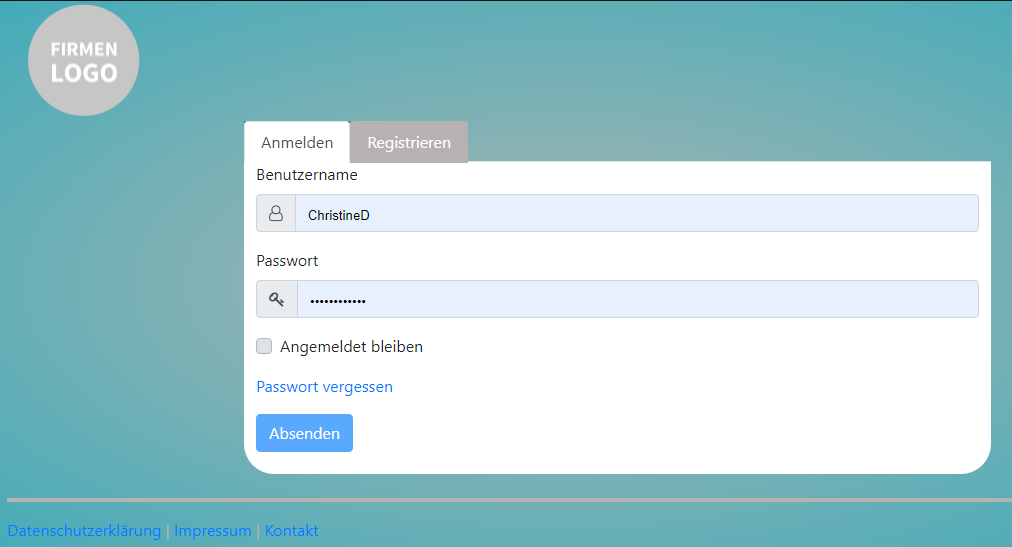
\includegraphics[width=1\textwidth,angle=0]{abb/login}
	\caption[Anmeldebildschirm]{Anmeldebildschirm}
	\label{fig:Anmeldebildschirm}
\end{figure}

Die~\ref{fig:Anmeldebildschirm} Abbildung zeigt den Anmeldebildschirm, dort können sich die Benutzer Anmelden und Registrieren.
\\
Ein weiterer Tipp von \cite{gui} wird hier umgesetzt, dieser heißt \glqq Orientiere dich an bereits erstellten Oberflächen\grqq{}. Vielen Anwendern ist die Struktur des Anmeldebildschirmes bereits von anderen Anwendungen bekannt, dadurch fällt Ihnen die Bedienung leichter, da sie vieles wiedererkennen.
\\
Sobald der JSON Web Token ungültig ist oder abgelaufen, wird der Nutzer immer auf den Anmeldebildschirm umgeleitet. Ein Token dient zur gegenseitigen Authentifizierung von Client und Server, erklärt \cite{token}. Sobald ein Benutzer sich zum ersten mal anmeldet, wird eine Anfrage (Request) an den Server gestellt. Dieser sendet eine Antwort (Response) zurück, sind die Anmeldedaten gültig, wird zusätzlich der Token mitgesendet. Der Token wird bei jeder erneuten Kommunikation mit dem Server mitgesendet.

\begin{figure}[htb]
	\centering
	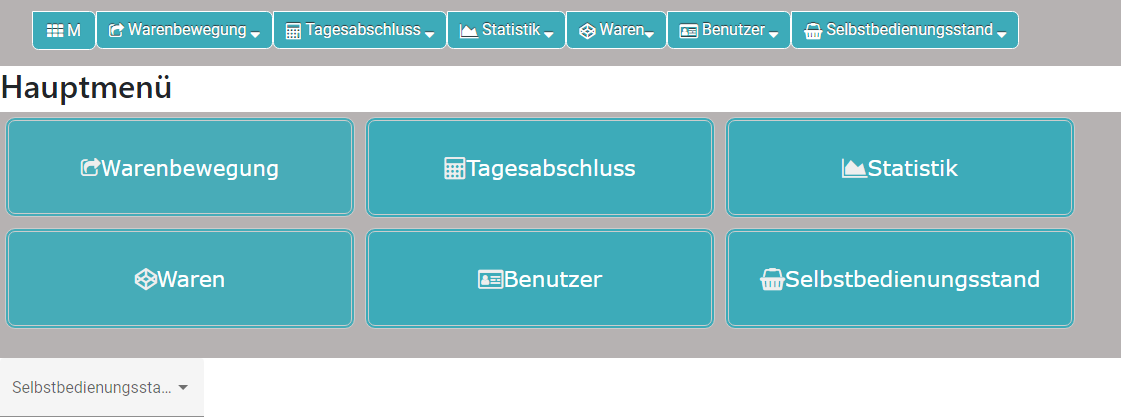
\includegraphics[width=1\textwidth,angle=0]{abb/hauptm}
	\caption[Hauptmenü]{Hauptmenü}
	\label{fig:Hauptmenü}
\end{figure}

Die Abbildung~\ref{fig:Hauptmenü} stellt das Hauptmenü da. Im oberen Bereich ist eine Navigationsleiste abgebildet, diese wird dauerhaft angezeigt. Der mittlere Bereich wird je nach Bedarf ausgetauscht. Im unteren Sektor kann der Anwender zwischen bestehenden Selbstbedienungsständen wechseln. 
\\
\\
Sobald der Nutzer den Punkt Warenbewegung auswählt, kann er dort die Warenbewegungen (Eingänge und Ausgänge) und das Datum eintragen.
\\
Ein Tagesabschluss wird erstellt, sobald der Anwender auf Tagesabschluss geht.
\\
Unter dem Menüpunkt Statistik sind Monats- und Jahresstatistiken zu finden.
\\
Mithilfe der Menüpunkte Waren, Benutzer und Selbstbedienungsstand können Waren, Benutzer und der Selbstbedienungsstand geändert, gelöscht oder hinzugefügt werden. 


\subsubsection{Entwurf des Hintergrundbereiches (Backend)}\label{entwurf_des_Hintergrundbereiches_(Backend)}

Die Ausgangsidee ist, die angefertigt Skizze des Hauptmenüs und des Anmeldebildschirmes, aus dem vorigen Kapitel, in einzelne Bestandteile bzw. Komponenten zu zerlegen.\\
 Die Abbildung ~\ref{fig:kompo} stellt dieses dar. 

\begin{figure}[htb]
	\centering
	\includegraphics[width=1\textwidth,angle=0]{abb/kompo}
	\caption[Darstellung der Komponenten des Clients]{Darstellung der Komponenten des Clients}
	\label{fig:kompo}
\end{figure}

Zu sehen ist der Hauptbereich~\ref{fig:kompo} unterteilt in einzelne Komponenten die jeweils farbig dargestellt sind. Die grün dargestellten Komponenten werden dauerhaft eingeblendet, dieses sind der Fußbereich, Hauptmenü und Auswahl des Selbstbedienungsstandes. 
\\
\\
Je nachdem in welchem Menü der Anwender sich befindet, wird im Hauptbereich (Gelb) situationsabhängig unterschiedliche Unterpunkte (Orange) angezeigt. Je nachdem, was der Benutzer davon auswählt, wird dieses im Hauptbereich eingeblendet.
\\
Dadurch ergibt sich folgende Struktur.
\begin{itemize}
	\itemsep0pt
	\item Hauptmenü
	\item Hauptbereich
		\subitem - Tagesabschluss 
			\subsubitem + Eintrag bearbeiten oder anlegen
			\subsubitem + Übersicht Tagesabschluss
		\subitem - Warenverwaltung 
			\subsubitem + Ware anlegen oder ändern
			\subsubitem + Übersicht Warenverwaltung
		\subitem - Warenbewegung 
			\subsubitem + Warenbewegung hinzufügen
			\subsubitem + Übersicht Warenverwaltung
			\subsubitem + Warenoptionen
		\subitem - Benutzerverwaltung 
			\subsubitem + Benutzerdaten bearbeiten
			\subsubitem + Übersicht Warenverwaltung
		\subitem - Selbstbedienungsstandverwaltung 
				\subsubitem + Selbstbedienungsstanddaten bearbeiten
				\subsubitem + Benutzer zum Selbstbedienungsstand hinzufügen
				\subsubitem + Benutzer anlegen und Selbstbedienungsstand hinzufügen
		\subitem - Statistik 
				\subsubitem + Monatsstatistik anzeigen
				\subsubitem + Jahresstatistik anzeigen
	\item Fußbereich
	\item Auswahl des Selbstbedienungsstandes
	
\end{itemize}


Zusätzlich werden unterschiedliche Serviceklassen angelegt, diese beinhalten Inhalte die von mehren unterschiedlichen Komponenten genutzt werden. 


